\documentclass[a4paper]{article}
\usepackage[utf8]{inputenc}
\usepackage[russian]{babel}
\usepackage[T2]{fontenc}
\usepackage[warn]{mathtext}
\usepackage{graphicx}
\usepackage{amsmath}
\usepackage{floatflt}
\usepackage{biblatex}       % for roman digits
\usepackage[left=20mm, top=20mm, right=20mm, bottom=20mm, footskip=10mm]{geometry}


\graphicspath{ {images/} }
\usepackage{multicol}
\setlength{\columnsep}{2cm}

\title{
    \textbf{Лабораторная работа 3.2.6}
}
\author{Герасименко Д.В.}
\date{2 курс ФРКТ, группа Б01-104}

\begin{document}
\maketitle

\begin{center}
    \raggedleft
        \underline{\underline{\LARGE {Аннотация}}}
\end{center}

\begin{center}
\raggedright
    \large{\textbf{Тема:}}
    \\
    \large {Изучение гальванометра}
    
    \large{\textbf{Цель работы:}}
    \\
    \large {Изучение работы высокочувствительного зеркального гальванометра магнитоэлектрической системы в режимах измерения постоянного тока и электрического заряда.}
    
    \large{\textbf{Оборудование:}}
    \\
    \large{Зеркальный гальванометр с осветителем и шкалой, источник постоянного напряжения, делитель напряжения, магазин сопротивлений, эталонный конденсатор, вольтметр, переключатель, ключи, линейка}
\end{center}

\begin{center}
    \raggedleft
        \underline{\underline{\LARGE {Теория}}}
\end{center}

\textit{Баллистический гальванометр} -- электроизмерительный прибор магнитоэлектрической системы, отличающийся высокой чувствительностью к току и сравнительно большим периодом свободных колебаний. \par
На помещённую в магнитное поле обтекаемую током рамку гальванометра действуют момент закрученной нити, момент магнитных сил и тормозящий момент (зависит от сил сопротивления воздуха и от вихревых токов). Учитывая все эти моменты, уравнение движения рамки принимает вид
\begin{equation}
    \ddot \varphi + 2 \gamma \dot \varphi + \omega_0^2\varphi = KI,
\end{equation}
где параметры колебательной системы:
\begin{equation*}
    K = \frac{BNS}{J}; \; 2\gamma = \beta_{\text{тр}} + \frac{(BNS)^{2}}{JR_{\Sigma}} \approx \frac{(BNS)^{2}}{JR_{\Sigma}}; \; \omega_{0}^{2} = \frac{D}{J}
\end{equation*}
$\gamma$ -- коэффициент затухания подвижной системы гальванометра, $\omega_0$ -- собственная частота колебаний рамки

Динамическая постоянная гальванометра (и обратная к ней величина - чувствительность) определяется при пропускании через рамку постоянного тока:

\begin{equation}
    C_{I} = \frac{I}{\varphi} = \frac{D}{BSN}; \; S_{I} = \frac{1}{C_{I}}
\end{equation}

где $B$ - индукция магнитного поля в рамке, $S$ - площадь одного витка рамки, $D$ - модуль кручения нити. \par
При пропускании коротких импульсов тока через баллистический гальванометр начальная скорость движения рамки пропорциональна электрическому заряду, прошедшему через рамку за всё время импульса. Отношение баллистических постоянных в критическом и свободном режимах равно $e$.

\newpage

\begin{center}
    \raggedleft
        \underline{\underline{\LARGE {Экспериментальная установка}}}
\end{center}

\begin{center}
    \underline{\large {\RN{1}. Определение динамической постоянной}}
\end{center}

\begin{figure}[h]
    \centering
    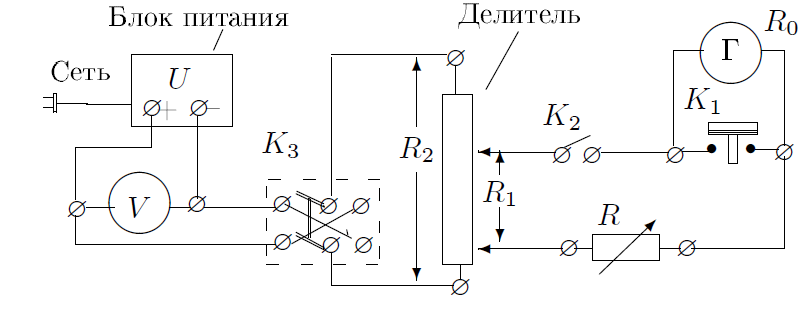
\includegraphics[width=11cm]{images/fig1.PNG}
    \caption{Схема установки для работы гальванометра в стационарном режиме}
    \label{fig:vac}
\end{figure}

Постоянное напряжение $U = 1,26$В снимается с блока питания и измеряется вольтметром $V$. Ключ $K_3$ позволяет менять величину тока через гальванометр Г, делитель напряжения - менять величину тока в широких пределах. Ключ $K_2$ служит для включения гальванометра, кнопка $K_1$ -- для его успокоения. Магазин сопротивлений $R$ позволяет менять режим работы гальванометра от колебательного до апериодического. \par
При малых $R_1$ сила тока, протекающего через гальванометр, может быть вычислена по формуле 
\begin{equation}
    I = U_0 \frac{R_1}{R_2} \frac{1}{R + R_0}.
\end{equation}
Динамическую постоянную вычисли по формуле 
\begin{equation}
    C_I = \frac{2aI}{x},
\end{equation}
где $a$ - расстояние от шкалы до зеркальца.

\begin{center}
    \underline{\large {\RN{2}. Определение критического сопротивления гальванометра}}
\end{center}

Выполняется с помощью той же цепи, что и на рис. 1. При больших $R$ движение рамки имеет колебательный характер, с уменьшением $R$ затухание увеличивается, и колебательный режим переходит в апериодический. Свяжем дикремент затухания колебаний с критическим сопротивлением. \par

В критическом режиме выполняется условие: \(\omega_{0} = \gamma\), откуда из ур-я (1) следует:

\begin{equation*}
    R_{\text{кр}} = R_{\Sigma_{\text{кр}}} - R_{0} = \frac{(BNS)^{2}}{2\sqrt{DJ}} - R_{0} = R_{\Sigma} \frac{\gamma}{\omega_{0}} - R_{0}
\end{equation*}

В колебательном режиме свободная частота колебаний: \(\omega_{1} = \sqrt{\omega_{0}^{2} - \gamma^{2}} = \frac{2\pi}{T_{1}}\).

Логарифмический декремент затухания:
\begin{equation*}
    \Theta = \ln{\frac{x_{n}}{x_{n+1}}} = \gamma T_{1} = 2\pi \frac{\gamma}{\sqrt{\omega_{0}^{2} - \gamma^{2}}} = 2\pi \frac{1}{\sqrt{\frac{\omega_{0}^{2}}{\gamma^{2}} - 1}} \rightarrow \frac{\gamma}{\omega_{0}} = \frac{1}{\sqrt{(\frac{2\pi}{\Theta})^{2} + 1}}
\end{equation*}

Подставляя это в уравнение выше и учитывая \(R_{\Sigma} = R + R_{0}\), получаем:
\begin{equation}
    R = \sqrt{\left(\frac{2\pi}{\Theta}\right)^{2} + 1} (R_{\text{кр}} + R_{0}) - R_{0} = (R_{\text{кр}} + R_{0}) \xi - R_{0} 
\end{equation}

Соответственно для определения критического сопротивления построим график зависимости \(R(\xi)\) и найдем значение углового коэффициента наклона прямой.

\newpage

\begin{center}
    \underline{\large {\RN{3}. Баллистической постоянная и критического сопротивления в баллистическом режиме}}
\end{center}

Для изучения работы гальванометра в режиме измерения заряда используется схема, представленная на рис. 2.

\begin{figure}[h]
    \centering
    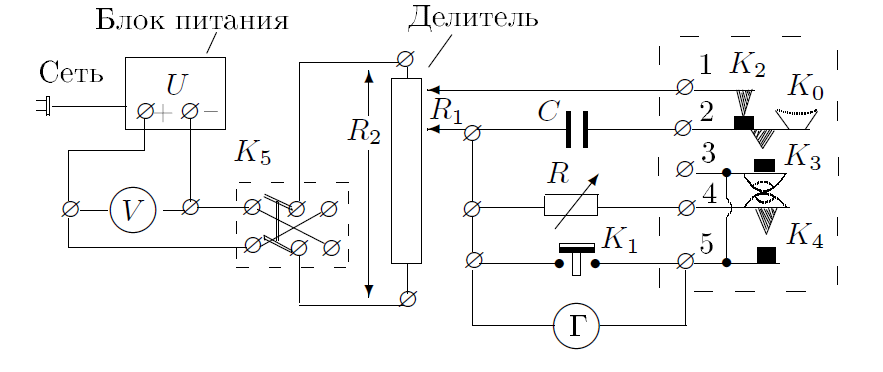
\includegraphics[width=10cm]{images/fig2.PNG}
    \caption{Схема установки для определения баллистической постоянной}
    \label{fig:vac}
\end{figure}

При нормальном положении кнопки $K_0$ конденсатор $C$ заряжается до напряжения
\begin{center}
    $U_c = \frac{R_1}{R_2}U_0$
\end{center}
Заряд конденсатора равен
\begin{center}
    $q = \frac{R_1}{R_2}U_0 C$
\end{center}

Проинтегрируем уравнение (1) по времени от 0 до \(\tau - \)
время протекания короткого импульса заряда. Пренебрегая значением угла отклоненя за это время, получим:

\begin{equation}
    \dot \varphi (\tau) = Kq \Rightarrow \varphi_{max} = \frac{\dot \varphi}{\omega_{0}} = \frac{Kq}{\omega_{0}}
\end{equation}

Но такое измерение трудно выполнить, так как необходимо добиться полного отсутствия затухания (свободный колебательный режим). Удобнее же всего измерять в критическом режиме: 
\begin{equation}
    \varphi(t) = \dot \varphi_{0}t\; e^{-\gamma t} \Rightarrow \dot \varphi(t_{o}) = 0 \Rightarrow t_{0} = \frac{1}{\gamma} \Rightarrow \varphi_{max}^{\text{кр}} =  \frac{1}{e} \frac{\dot \varphi_{0}}{\gamma} =  \frac{1}{e} \frac{\dot \varphi_{0}}{\omega_{0}} = \frac{\varphi_{max}^{\text{св}}}{e}
\end{equation}

В нём максимальное отклонение в \(e\) раз меньше, чем при случае свободных колебаний

Характеристика \(C_{q} = \frac{q}{\varphi_{max}}\) называется баллистической постоянной гальванометра. В критическом режиме 

\begin{equation}
    C_{q_{\text{кр}}} = \frac{q}{\varphi_{max}^{\text{кр}}} = 2a\frac{R_1}{R_2} \frac{U_0 C}{l_{max}^{\text{кр}}}
\end{equation}

где \(x_{max} - \) максимальное отклонение зайчика при разомкнутой внешней цепи (\(R = \infty\)), a - расстояние от зеркальца до шкалы

\begin{center}
    \raggedleft
        \underline{\underline{\LARGE {Выполнение}}}
\end{center}

\begin{enumerate}
    \item Подготовим к работе приборы, настроим гальванометр. Соберём схему согласно рис. 1. Снимем зависимость отклонения зайчика $x$ от сопротивления магазина $R$, увеличивая сопротивление магазина, но не меняя делителя. Результаты запишем в табл. 1. Ток в цепи рассчитаем по формуле (1) ($R_1/R_2 = 1/2000$, $U_0 = 1.26$ В, $R_0 = 610$ Ом.)
    
\begin{center}
    \textbf{Таблица 1.} Зависимость отклонения зайчика от сопротивления при постоянном токе

    \begin{tabular}{|c|c|c|c|c|c|c|c|c|}
        \hline
        $x$, мм & 254 & 213 & 183 & 161 & 143 & 129 & 117 & 108 \\
        \hline
        $R$, кОм & 2.0 & 2.5 & 3.0 & 3.5 & 4.0 & 4.5 & 5.0 & 5.5 \\
        \hline
        $I$, нА & 241.38 & 202.57 & 174.52 & 153.28 & 136.66 & 123.29 & 112.30 & 103.11 \\
        \hline
    \end{tabular}

    \begin{tabular}{|c|c|c|c|c|c|c|c|c|}
        \hline
        $x$, мм & 100 & 92 & 86 &81 & 77 & 72 & 68 & 65 \\
        \hline
        $R$, кОм & 6.0 & 6.5 & 7.0 & 7.5 & 8.0 & 8.5 & 9.0 & 9.5 \\
        \hline
        $I$, нА & 95.31 & 88.61 & 82.79 & 77.68 & 73.17 & 69.15 & 65.56 & 62.31 \\
        \hline
    \end{tabular}  
\end{center}

Графически представим результаты на графике $I = f(x)$ (рис. 3). Воcпользуемся методом наименьших квадратов для определения наклона прямой и погрешности его определения.  

\begin{figure}[h]
    \centering
    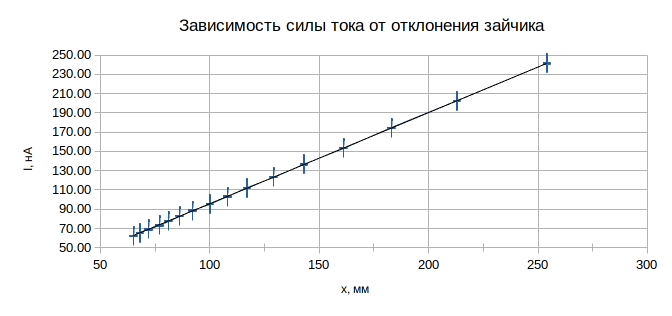
\includegraphics[width=\textwidth]{images/graph1.PNG}
    \caption{Определение динамической постоянной гальванометра}
    \label{fig:vac}
\end{figure}

\begin{equation}
    C_{I} = 2.57 \; \frac{\text{нА}}{\text{мм}/\text{м}} \;
    \sigma_{C_{I}} = 0.02 \; \frac{\text{нА}}{\text{мм}/\text{м}}
\end{equation}

Итого получаем
\begin{center}
    $C_I = 2.57 \pm 0.02$ нА/(мм/м) \\
    $S_I = 0.39 \pm 0.01$ \(\text{нА/(мм/м)}^{-1}\)
\end{center}

\item Рассчитаем логарифмический декремент затухания свободных колебаний рамки разомкнутого гальванометра. Результаты измерений занесём в табл. 2. Также определим приблизительно период свободных колебаний рамки.


\begin{center}
    \begin{tabular}{|c|c|c|c|c|c|c|c|c|c|c|c|c|c|}
        \hline
        \(x_{1}\), мм & \(x_{2}\), мм & \(x_{3}\), мм & \(x_{4}\), мм & \(x_{5}\), мм & \(\Theta_{12}\) & \(\Theta_{23}\) & \(\Theta_{34}\) & \(\Theta_{45}\) & \(\Theta\) & \(\sigma_{\Theta}\) &T, с \\
        \hline
        254 & 212 & 179 & 150 & 126 & 0.180 & 0.169 & 0.176 & 0.174 & 0.174 & 0.002 & 2.8 \\
        \hline
    \end{tabular}   
    
    \textbf{Таблица 2.} Для определения декремента затухания
\end{center}


Получили значение логарифмического декремента затухания свободных колебаний рамки
\begin{center}
   $\Theta = 0.174 \pm 0.002$ 
\end{center}

\item При разомкнутом ключе $K_3$ определим наибольшее сопротивление магазина $R$, при котором при размыкании ключа зайчик не переходит за нулевое значение шкалы. Это сопротивление близко к критическому $R_c_r \approx 7.3$ кОм.

\item Установим сопротивление магазина $R \approx 3R_c_r$ и подберем делитель так, чтобы в стационарном режиме зайчик отклонялся на всю шкалу. Для расчёта $\Theta$ будем измерять два последовательных отклонения зайчика в одну сторону. Повторим измерения, увеличивая сопротивление магазина до $10R_c_r$. Результаты занесём в табл. 3.

\newpage

\begin{table}[h]
    \centering
    \begin{center}
        \textbf{Таблица 3.} Зависимость отклонения зайчика от сопротивления, после размыкания ключа $K_3$
    \end{center}
    \label{tab:my_label}
    \begin{tabular}{|p{1.5cm}||p{0.8cm}|p{0.8cm}|p{0.8cm}|p{0.8cm}|p{0.8cm}|p{0.8cm}|p{0.8cm}|p{0.8cm}|p{0.8cm}|p{0.8cm}|p{0.8cm}| }
        \hline
            $R$, кОм & 3.0 & 3.5 & 4.0 & 4.5 & 5.0 & 5.5 & 6.0 & 7.0 & 8.0 & 9.0 & 10.0 \\
        \hline
            $x1$, мм & 250 & 216 & 188 & 167 & 149 & 132 & 124 & 1106 & 93 & 84 & 75 \\
        \hline
            $x2$, мм & 38 & 42 & 44 & 45 & 44 & 44 & 45 & 43 & 41 & 39 & 36 \\
        \hline
            $\Theta$ & 1.884 & 1.636 & 1.452 & 1.311 & 1.220 & 1.121 & 1.014 & 0.902 & 0.819 & 0.767 & 0.734 \\
        \hline
            $\xi$ & 3.48 & 3.96 & 4.44 & 4.89 & 5.24 & 5.69 & 6.28 & 7.03 & 7.73 & 8.25 & 8.61 \\
        \hline
    \end{tabular}
\end{table}   

Построим график зависимости декремента затухания колебаний от сопротивления на магазине в координатах $R(\xi)$ (рис. 4). Используя формулу (4) и метод наименьших квадратов, определим по нему критическое сопротивление гальванометра. Также используя метода наименьших квадратов, оценим погрешность определения этой величины (так как погрешность измерения отклонения зайчика пренебрежимо мала по сравнению с погрешностью по МНК): \(k = 9.5\) кОм; \(\sigma_{k} = 0.4\) кОм; \(\frac{\sigma_{k}}{k} = 4.2 \%\)

\begin{figure}[h]
    \centering
    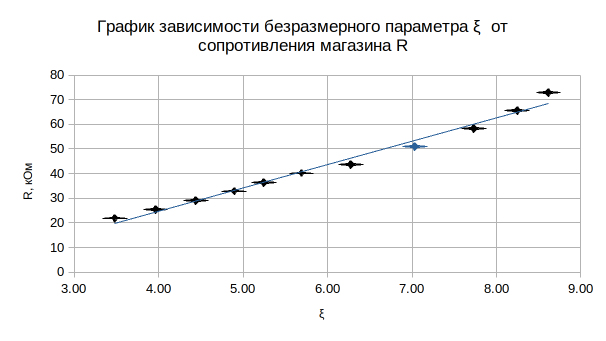
\includegraphics[width=0.8\textwidth]{images/graph2.PNG}
\end{figure}

Откуда получим значение критического сопротивления в данном методе:

\begin{center}
    \(R_{\text{кр}} = 8.9 \pm 0.4\) кОм
\end{center}


\item Перейдём к работе гальванометра в баллистическом режиме. Соберём схему по рис. 2. Разомкнём цепь $R$, отсоединив одну из клемм от магазина. Подберём делитель так, чтобы первый отбор соответствовал отклонению зайчика на всю школу. Для свободных колебаний $l_{max} = 203$ мм. \par
Подключим магазин назад. Снимем зависимость величины первого отброса от $R$. Результаты занесём в табл. 4.


\begin{table}[h]
    \centering
    \begin{center}
        \textbf{Таблица 4.} Зависимость максимального отклонения зайчика от сопротивления внешней части цепи в режиме измерения заряда
    \end{center}
    \begin{tabular}{ |p{1.5cm}||p{1cm}|p{1cm}|p{1cm}|p{1cm}|p{1cm}|p{1cm}|}
\hline

    $l_{max}$, мм & 169 & 166 & 152 & 137 & 102 & 67 \\
\hline
    $R$, кОм & 50 & 40 & 30 & 20 & 10 & 5 \\
\hline

    \end{tabular}
\end{table} 

Построим график $l_{max} = f[(R_0 + R)^{-1}]$. По графику, используя метод наименьших квадратов, определим критическое сопротивление гальванометра (\(l_{\text{кр}} = l_{max}/e\)). 
Для уравнения \(l_{max} = kt + l\), получим

\begin{figure}[h]
    \centering
    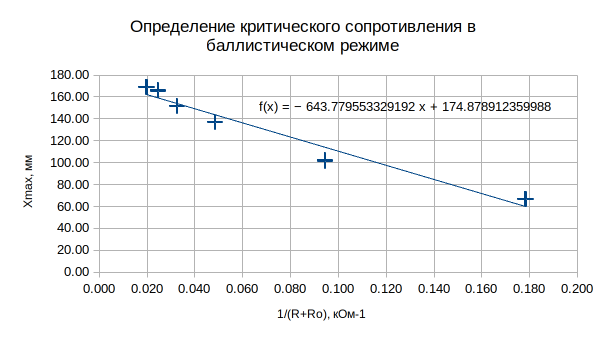
\includegraphics[width=0.8\textwidth]{images/graph3.PNG}
\end{figure}

\begin{center}
    \(k = -643 \text{кОм мм}^{-1}; l = 174 \text{мм}\) \par
    \(\sigma_{k} = 106 \text{кОм мм}^{-1}; \sigma_{l} = 9 \text{мм} \) \par
    \(R_{\text{кр}} = \left(\frac{l_{\text{кр}} - l}{k}\right)^{-1} - R_0 = (5.9 \pm 0.9)\) кОм
\end{center}

\item По формуле (5) рассчитаем баллистическую постоянную в критическом режиме:

\begin{center}
    \(C_{q}^{\text{кр}} = 2a\frac{R_{1}}{R_{2}}\frac{CU_{0}}{l_{max}^{\text{кр}}}\); \(\frac{\sigma_{C_{q}^{\text{кр}}}}{C_{q}^{\text{кр}}} = \frac{\sigma{l_{max}}}{l_{max}}\) \par
    
    \(C_{q}^{\text{кр}} = (1.71 \pm 0.02) \; 10^{-9}\) К / (мм/м)
\end{center}

\item Сравним время релаксации $t = R_0 C$ и период свободных колебаний гальванометра $T_0$
\begin{center}
    $t = 5.2 \cdot 10^{-6} c \ll T = 2.6 c$
\end{center}
Время релаксации много меньше периода свободных колебаний. Эксперимент корректен.

\end{enumerate}

\begin{center}
    \raggedleft
        \underline{\underline{\LARGE {Вывод}}}
\end{center}

В ходе эксперимента был исследован принцип работы гальванометра в режиме постоянного тока и в баллистическом режиме. Определены динамическая и баллистическая постоянные гальванометра:

\begin{center}
    $C_I = (2.57 \pm 0.02)$ нА/(мм/м) \hspace{1cm} $C_{q}^{\text{кр}} = (1.71 \pm 0.02) \cdot 10^-^9$ К/(мм/м)
\end{center}

Тремя разными способами было исследовано критическое сопротивление гальванометра. Результаты отличны в пределах погрешности.

\begin{table}[h]
    \centering
    \begin{center}
        \textbf{Таблица 5.} Значения $R_c_r$, полученные разными способами
    \end{center}
    \begin{tabular}{ |p{4cm}|p{4cm}|p{4cm}|}
    \hline
        $R_c_r$, кОм - подбор & $R_c_r$, кОм  - по графику в стационарном режиме & $R_c_r$, кОм - по графику в баллистическом режиме \\
    \hline
        $7.3$ & $8.9 \pm 0.4$ & $5.9 \pm 0.9$ \\
    \hline
    \end{tabular}
\end{table} 

Наиболее точным считаем значение сопротивления, которое было измерено в режиме постоянного тока по следующей причине: эксперимент в баллистическом режиме менее точен ввиду больших требований к установке (необходимо достичь максимальную чувствительность гальванометра к заряду и сократить время, затрачиваемое на измерение).

\end{document}